%%%%%%%%%%%%%%%%%%%%%%%%%%%%%%%%%%%%%%%%%%%%%%%%%%%%%%%%%%%%%%%%%%%%%%%%%%%%%%%%
% Template for USENIX papers.
%
% History:
%
% - TEMPLATE for Usenix papers, specifically to meet requirements of
%   USENIX '05. originally a template for producing IEEE-format
%   articles using LaTeX. written by Matthew Ward, CS Department,
%   Worcester Polytechnic Institute. adapted by David Beazley for his
%   excellent SWIG paper in Proceedings, Tcl 96. turned into a
%   smartass generic template by De Clarke, with thanks to both the
%   above pioneers. Use at your own risk. Complaints to /dev/null.
%   Make it two column with no page numbering, default is 10 point.
%
% - Munged by Fred Douglis <douglis@research.att.com> 10/97 to
%   separate the .sty file from the LaTeX source template, so that
%   people can more easily include the .sty file into an existing
%   document. Also changed to more closely follow the style guidelines
%   as represented by the Word sample file.
%
% - Note that since 2010, USENIX does not require endnotes. If you
%   want foot of page notes, don't include the endnotes package in the
%   usepackage command, below.
% - This version uses the latex2e styles, not the very ancient 2.09
%   stuff.
%
% - Updated July 2018: Text block size changed from 6.5" to 7"
%
% - Updated Dec 2018 for ATC'19:
%
%   * Revised text to pass HotCRP's auto-formatting check, with
%     hotcrp.settings.submission_form.body_font_size=10pt, and
%     hotcrp.settings.submission_form.line_height=12pt
%
%   * Switched from \endnote-s to \footnote-s to match Usenix's policy.
%
%   * \section* => \begin{abstract} ... \end{abstract}
%
%   * Make template self-contained in terms of bibtex entires, to allow
%     this file to be compiled. (And changing refs style to 'plain'.)
%
%   * Make template self-contained in terms of figures, to
%     allow this file to be compiled. 
%
%   * Added packages for hyperref, embedding fonts, and improving
%     appearance.
%   
%   * Removed outdated text.
%
%%%%%%%%%%%%%%%%%%%%%%%%%%%%%%%%%%%%%%%%%%%%%%%%%%%%%%%%%%%%%%%%%%%%%%%%%%%%%%%%

\documentclass[letterpaper,twocolumn,10pt]{article}
\usepackage{usenix-2020-09}

% to be able to draw some self-contained figs
\usepackage{tikz}
\usepackage{amsmath}
\usepackage{float}
% inlined bib file
\usepackage{filecontents}
\usepackage{enumitem}
%-------------------------------------------------------------------------------
\begin{filecontents}{\jobname.bib}
%-------------------------------------------------------------------------------
@Book{arpachiDusseau18:osbook,
  author =       {Arpaci-Dusseau, Remzi H. and Arpaci-Dusseau Andrea C.},
  title =        {Operating Systems: Three Easy Pieces},
  publisher =    {Arpaci-Dusseau Books, LLC},
  year =         2015,
  edition =      {1.00},
  note =         {\url{http://pages.cs.wisc.edu/~remzi/OSTEP/}}
}
@InProceedings{waldspurger02,
  author =       {Waldspurger, Carl A.},
  title =        {Memory resource management in {VMware ESX} server},
  booktitle =    {USENIX Symposium on Operating System Design and
                  Implementation (OSDI)},
  year =         2002,
  pages =        {181--194},
  note =         {\url{https://www.usenix.org/legacy/event/osdi02/tech/waldspurger/waldspurger.pdf}}}
\end{filecontents}

%-------------------------------------------------------------------------------
\begin{document}
%-------------------------------------------------------------------------------

%don't want date printed
\date{}

% make title bold and 14 pt font (Latex default is non-bold, 16 pt)
\title{\Large \bf Seminar Report: \\
HyperEnclave: An Open and Cross-platform Trusted Execution Environment}

%for single author (just remove % characters)
\author{
{\rm Ahmet Turkmen}\\
Technical University of Munich
\and
{\rm Mert Sarac}\\
Technical University of Munich
% copy the following lines to add more authors
% \and
% {\rm Name}\\
%Name Institution
} % end author

\maketitle

%-------------------------------------------------------------------------------
% 
\begin{abstract}
% %-------------------------------------------------------------------------------
% Your abstract text goes here. Just a few facts. Whet our appetites.
% Not more than 200 words, if possible, and preferably closer to 150.
% 

\end{abstract}


%-------------------------------------------------------------------------------
\section{Introduction and Problem Definition}
%-------------------------------------------------------------------------------

An enclave is a secure and isolated environment within a larger network or infrastructure that is designed to protect sensitive or classified information. These enclaves prevent unauthorized access to the information stored within them and detect and respond to any attempts at intrusion. They are isolated from larger networks or infrastructure through dedicated hardware or software, or by physically separating the enclave from the rest of the network. Beyond traditional security measures, enclave technology offers additional levels of protection such as firewalls and encryption. Despite their high level of security, this technology also has some drawbacks. Existing trusted execution environments (TEEs) are bound to specific vendors such as Intel, AMD, ARM, and IBM. This limits enclaves to adapt to diverse workloads. Also, they are closed source which excludes the research community to audit them. In addition, current TEEs lack supporting commodity hardware without hardware or firmware changes. *** Another drawback is that most TEE design enforces enclaves run in a fixed mode. It is difficult to meet the performance and security requirements of various applications. Finally, they are not invulnerable to all attacks even if they provide a high level of security.

Opposed to that, a solution named “HyperEnclave” is proposed which is an open source, cross-platform TEE with multiple flexible running modes. It offers an invulnerability to some specific attacks such as memory mapping attacks that current TEEs cannot handle. 

In this paper, a detailed overview and analysis about Hyper Enclave will be mentioned.


%-------------------------------------------------------------------------------
\section{Background Information}
%-------------------------------------------------------------------------------
A trusted execution environment (TEE) is a processing environment which is isolated, secure, and integrity protected that includes processing, memory, and storage capabilities. [Trusted Execution Environments on Mobile Devices]
Being isolated makes TEEs invulnerable for most malicious actors to access and tamper with sensitive data.

%-------------------------------------------------------------------------------
\section{Analysis of Current Work}

\begin{description}
  
\item[fread] a function that reads from a \texttt{stream} into the
  array \texttt{ptr} at most \texttt{nobj} objects of size
  \texttt{size}, returning returns the number of objects read.

\item[Fred] a person's name, e.g., there once was a dude named Fred
  who separated usenix.sty from this file to allow for easy
  inclusion.
\end{description}

\noindent
The noindent at the start of this paragraph in its tex version makes
it clear that it's a continuation of the preceding paragraph, as
opposed to a new paragraph in its own right.



%----------------------------------------------------------------------------
\subsection{Importance and Challanges}
%-----------------------------------
Due to increasing privacy and security concerns TEEs are becoming crucial, since sensitive information is being stored and processed through devices. However, adaptation of TEEs on diverse workloads is not trivial and requires high engineering effort. Moreover, current TEEs are subject to exploit page attacks. The challenges can be summarized in points as follows: 
\begin{itemize}
    \item The need for minimal code base in the TCB
    \item The need to build TEEs that can run on commodity hardware without hardware or firmware changes.
    \item The need for non-trivial engineering effort to adapt HyperEnclave to other platforms such as ARM and RISC-V due to differences in instruction set architectures (ISAs).
    \item The need to minimize the attack surfaces under different enclave operation modes.
\end{itemize}




%----------------------------------------------------------------------------
\subsection{System Overview}
%----------------------------------------------------------------------------
HyperEnclave has three main design goals which are; minimum hardware requirements, easy to develop, flexible enclave modes. Minimum hardware requirements goal provided through hardware virtualization and by using the Trusted Platform Module (TPM) to provide a root of trust for the system. Easy to develop, HyperEnclave is SGX compatible, it means that porting existing SGX programs does not lead to overhead.
\newline
Overall overview of HyperEnclave can be seen in Figure 1. 
\begin{figure}[H]
    \centerline{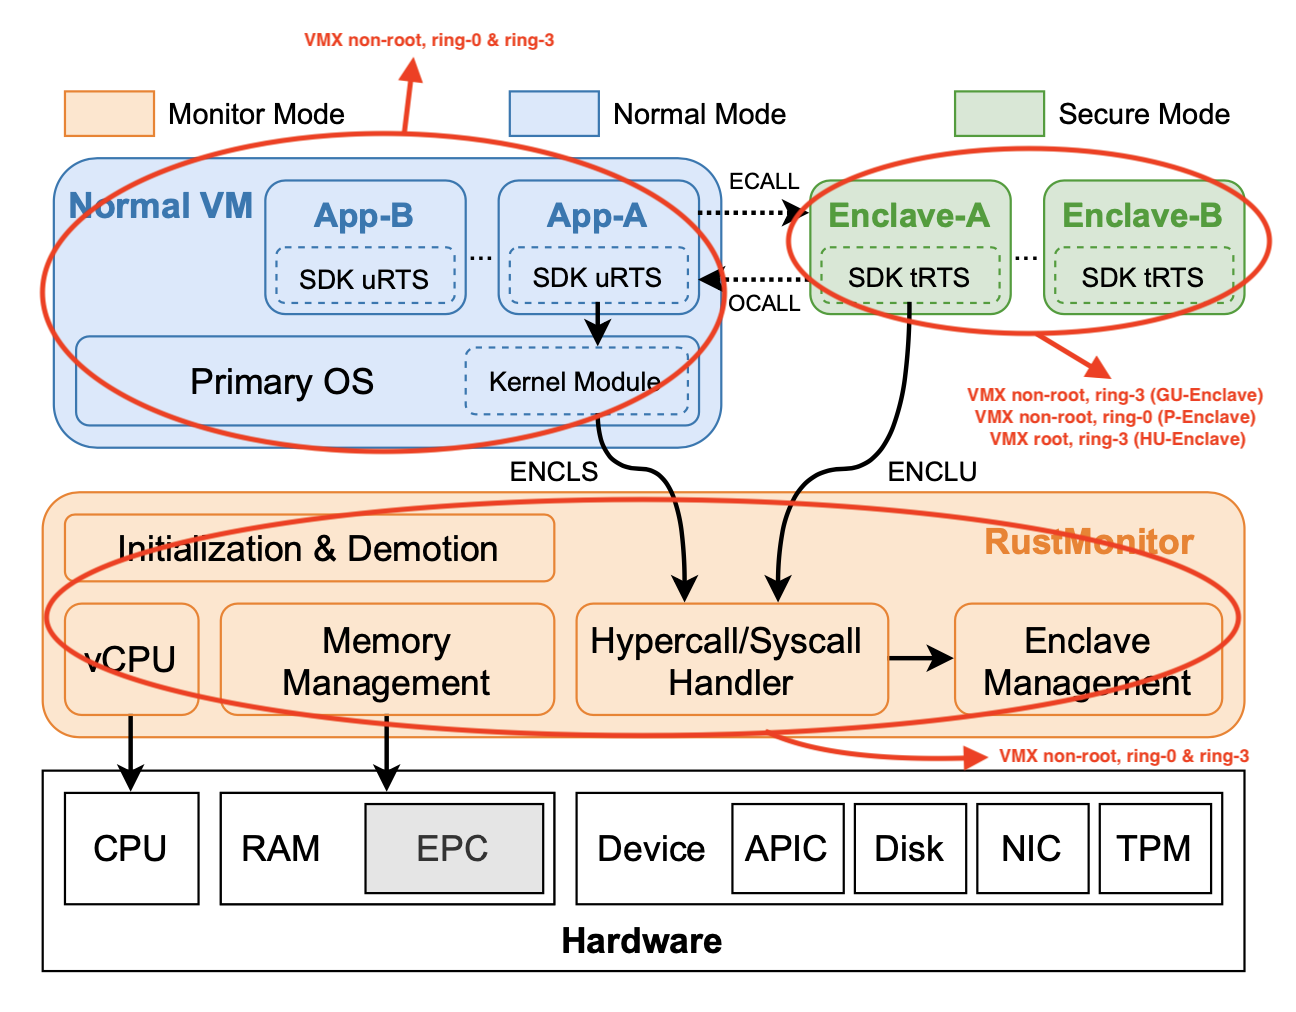
\includegraphics[scale=.42]{figures/system_overview.png}}
    \caption{System Overview}
    \label{fig}
\end{figure}

HyperEnclave is a Trusted Execution Environment (TEE) that allows for the creation of flexible enclaves on commodity hardware without requiring any hardware or firmware changes. HyperEnclave uses hardware virtualization features such as two-level address translation and TPM for the root of trust and randomness.
Multiple modes of operation supported as seen in given Figure 1, including the monitor mode, normal mode, and secure mode. Secure mode has different capabilities to run in a variety of VMx permissions, at ring 3 (GU Enclave) and at ring 0 (P Enclave) it can run in non-root mode in addition, at ring 3 (HU Enclave) runs in root mode. Normal mode only supports non-root modes which are at ring 0 and ring 3 as illustrated in the Figure. Similarly Rustmonitor runs in VMX non-root mode at ring 0 and ring 3. 

It consists of several components, including the RustMonitor, a lightweight hypervisor that manages the enclave memory and controls the enclave state transitions. The primary OS (such as Linux) and untrusted part of applications that run in the normal mode.  A kernel module in the primary OS for loading and launching RustMonitor. HyperEnclave SDK compatible with  Intel SGX SDK hence allows for easy development and most SGX programs can run on HyperEnclave with minimal changes to the source code. HyperEnclave is prototyped on AMD servers.
HyperEnclave modes can be summarized through Figure 2. 

\begin{figure}[H]
    \centerline{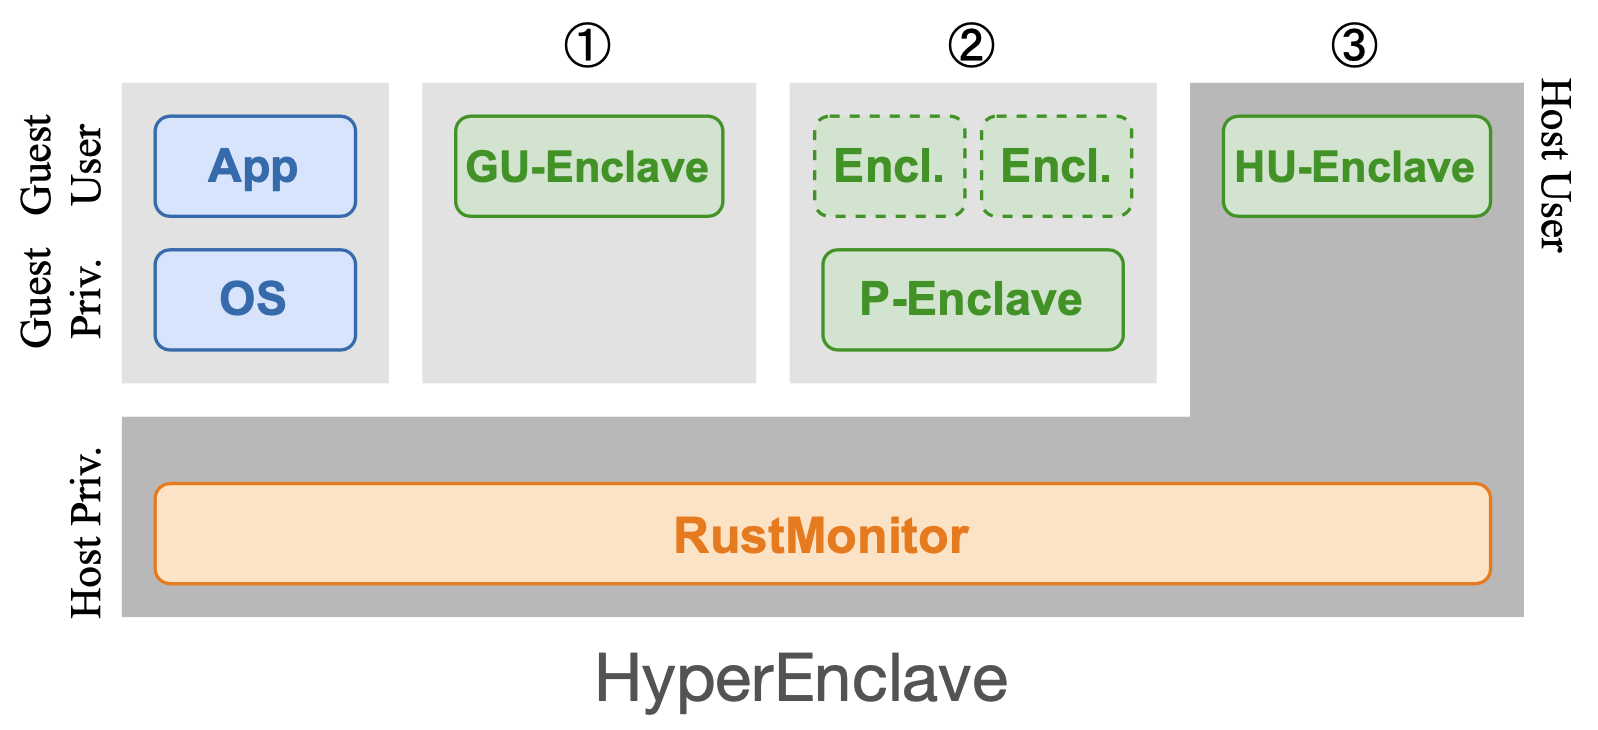
\includegraphics[scale=.15]{figures/hyperenclave_modes.png}}
    \caption{HyperEnclave modes}
    \label{fig}
\end{figure}


\begin{enumerate}[topsep=0pt, partopsep=0pt]
    \setlength\itemsep{-0.4em}
    \item GU-Enclave - basic enclave operation mode, it is used for computing intensive workloads and running in guest user mode. 
    \item P-Enclave -  privileged enclaves are running in privileged guest user mode, have access to IDT, page tables and level 1 page tables. Garbage collectors (essential in Java)  are using P-Enclave privileges. 
    \item HU-Enclave  -  running in host user mode,  provides fast world switches (according to experiments in the paper ) hypercalls: ∼ 880 CPU and syscalls: ∼ 120 CPU cycles. HU-Enclave is preferred for I/O intensive workloads
\end{enumerate}

%----------------------------------------------------------------------------



%----------------------------------------------------------------------------
\subsection{Evaluation}
%----------------------------------------------------------------------------
HyperEnclave is evaluated on several applications namely a lightweight web server Lighttpd and Redis  which are CPU-Intensive and memory-intensive tasks in order. The evaluations were conducted by porting the OS Occlum library to the enclave SDK, and measuring the performance on both HyperEnclave and Intel SGX. The experiments show that HyperEnclave has a lower overhead than SGX, and performs better on memory-intensive tasks as shown in Figure 3 .

\begin{figure}[H]
    \centerline{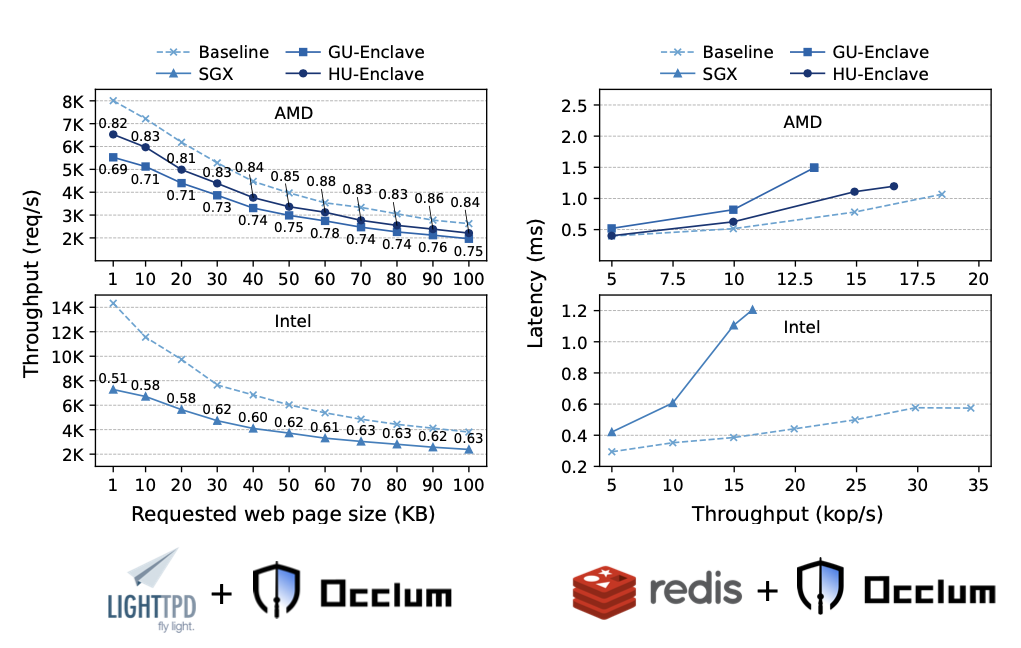
\includegraphics[scale=.30]{figures/evaluation.png}}
    \caption{Evaluation results on lighttpd+occlum and redis+occlum}
    \label{fig}
\end{figure}

 Additionally, the performance of HyperEnclave in HU-Enclave mode is better than that of SGX in most cases. Overall, the results suggest that HyperEnclave is a promising technology for secure data processing.



%----------------------------------------------------------------------------
\section{Discussion}
%-------------------------------------------------------------------------------

The USENIX latex style is old and very tired, which is why
there's no \textbackslash{}acks command for you to use when
acknowledging. Sorry.

%-------------------------------------------------------------------------------
\section*{Conclusion}
%-------------------------------------------------------------------------------

USENIX program committees give extra points to submissions that are
backed by artifacts that are publicly available. If you made your code
or data available, it's worth mentioning this fact in a dedicated
section.

%-------------------------------------------------------------------------------
\bibliographystyle{plain}
\bibliography{\jobname}

%%%%%%%%%%%%%%%%%%%%%%%%%%%%%%%%%%%%%%%%%%%%%%%%%%%%%%%%%%%%%%%%%%%%%%%%%%%%%%%%
\end{document}
%%%%%%%%%%%%%%%%%%%%%%%%%%%%%%%%%%%%%%%%%%%%%%%%%%%%%%%%%%%%%%%%%%%%%%%%%%%%%%%%

%%  LocalWords:  endnotes includegraphics fread ptr nobj noindent
%%  LocalWords:  pdflatex acks